\documentclass[border=3mm]{standalone}
\usepackage{pgfplots, amsmath}

\begin{document}

 
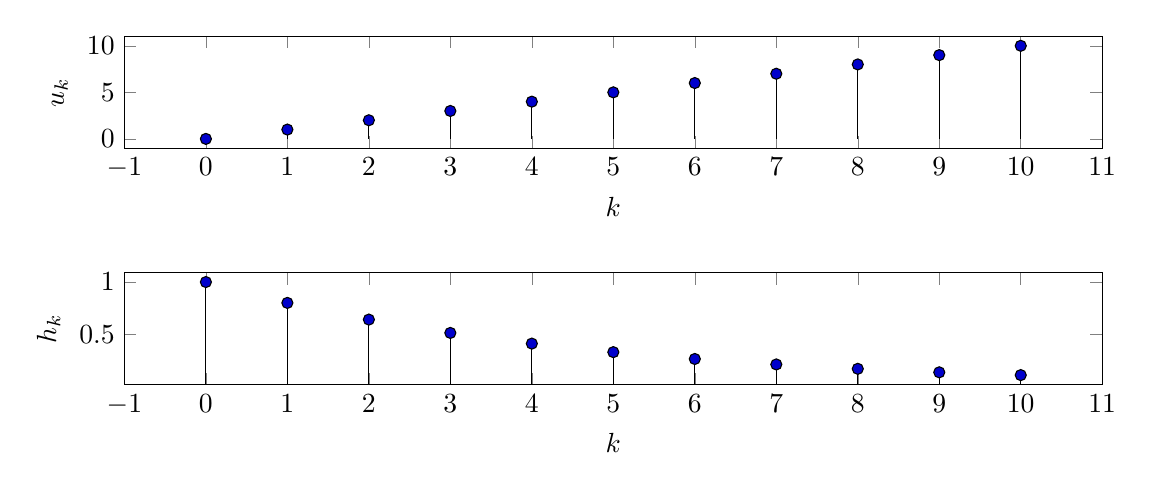
\begin{tikzpicture}
\begin{axis}[
  width=14cm,
  height=3cm,
  xlabel={$k$},
  ylabel={$u_k$},
]

%\addplot+[black, ycomb, domain=0:40, samples=41,variable=k] {pow(0.9, k)*cos(deg(3.1415/5*k))}; 
\addplot+[black, ycomb, domain=0:10, samples=11,variable=k] {k}; 

\end{axis}
\begin{axis}[
  width=14cm,
  height=3cm,
  yshift=-3cm,
  xlabel={$k$},
  ylabel={$h_k$},
]

\addplot+[black, ycomb, domain=0:10, samples=11,variable=k] {pow(0.8, k)}; 

\end{axis}
\end{tikzpicture}
\end{document}